\documentclass{article}
\usepackage{amsmath}
\usepackage{hyperref}
\usepackage{amssymb}
\usepackage{graphicx}
\usepackage{float}
\usepackage{bm}
\usepackage[top=2cm]{geometry}
\renewcommand{\thesubsubsection}{\thesubsection\ \alph{subsubsection})}

\title{Deep Learning - Homework 1}
\author{99222 - Frederico Silva, 99326 - Sebastião Carvalho}
\date{\today}

\begin{document}

\maketitle

\tableofcontents

\section{Question 1}

Medical image classification with linear classifiers and neural networks.

\subsection{}

\subsubsection{}

\paragraph{Answer} After running the code, the following plot was generated:
\begin{figure}[H]
    \centering
    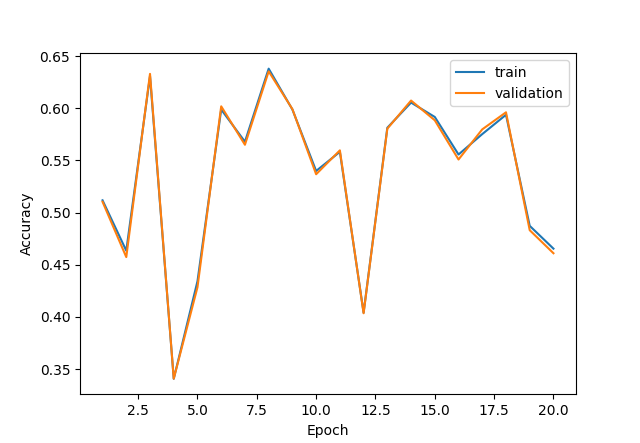
\includegraphics[width=0.8\textwidth]{"plots/1_1_a.png"}
    \caption{Perceptron Training and Validation Accuracy}
    \label{1.1.a Plot}
\end{figure}

The test accuracy was 0.3422.

\subsubsection{}
\paragraph{Answer} After running the code, the following plots were generated for learning rates $\eta = 0.01$ and $\eta = 0.001$, respectively:
\begin{figure}[H]
    \centering
    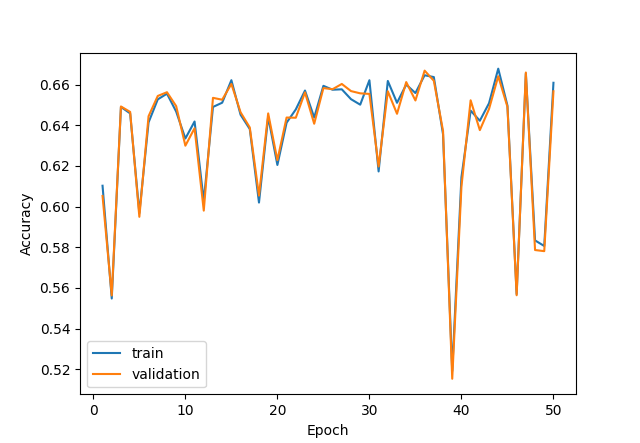
\includegraphics[width=0.8\textwidth]{"plots/1_1_b_001.png"}
    \caption{Logistic Regression Accuracy with Learning Rate $\eta = 0.01$}
    \label{1.1.b 0.01 Plot}
\end{figure}

\begin{figure}[H]
    \centering
    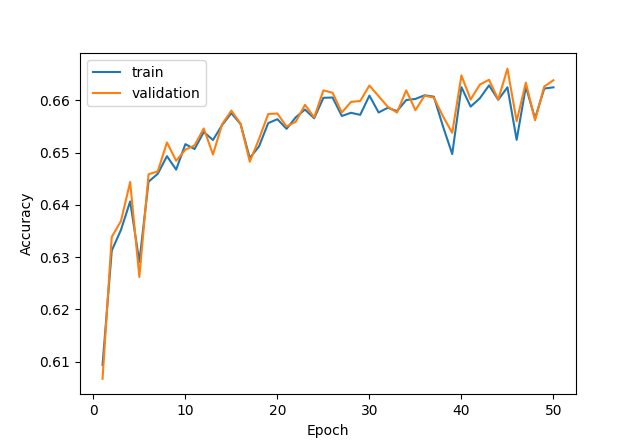
\includegraphics[width=0.8\textwidth]{"plots/1_1_b_0001.png"}
    \caption{Logistic Regression Accuracy with Learning Rate $\eta= 0.001$}
    \label{1.1.b 0.0001 Plot}
\end{figure}

The test accuracy was 0.5784 and 0.5936 for $\eta = 0.01$ and $\eta = 0.001$ respectively.\\
Comparing both charts, we can see that for $\eta = 0.001$, the accuracy increases more slowly, but it reaches a higher value than for $\eta = 0.01$. 
This is because for $\eta = 0.01$, the algorithm is taking too big steps, and it is not able to converge to a better solution. This can be 
seen in the chart for $\eta = 0.01$, near epoch 40, when the accuracy drops to an all time low.\\
Since the learning rate is too small for $\eta = 0.001$, the algorithm takes longer to reach higher accuracies, but it's also 
less oscillatory, and it is able to converge to a better solution.\\

\subsection{}

\subsubsection{}

\paragraph{Answer}
The answer to this question mainly focus on two topics: how complex the models are, meaning their expressiveness, and how easy they are to train. \\
Regarding the expressiveness, logistic regression is a linear model that learns a single decision boundary to separate classes. 
When using pixel values as features, it treats each pixel independently and cannot capture complex patterns such as shapes or textures 
that might be essential for tasks like image classification.\\ 
On the other hand, a multi-layer perceptron can learn non-linear decision boundaries due to its hidden layers and non-linear activation functions like ReLU. 
Each layer can transform the feature space in a way that makes the data linearly separable by subsequent layers, allowing the MLP to capture 
complex patterns and relationships in the data.\\
When it comes to how easy it is to train this models, logistic regression, with its convex cost function, offers a straightforward training guaranteed 
to reach the global minimum, given enough time and proper learning hyperparameters. 
However, when talking of a multi-layer perceptron, the presence of multiple layers and non-linearities in an MLP makes the optimization landscape non-convex. 
There can be multiple local minima, saddle points, and plateaus. Finding the global minimum is not guaranteed, making the training process, 
most of the times, more complex.\\
In short, the claim is true. A logistic regression model is less expressive than a multi-layer perceptron with ReLU activations because it can only 
represent linear relationships, whereas MLPs can capture non-linearities. Logistic regression models are easier to train because they involve 
convex optimization, unlike the non-convex problem of training MLPs.

\subsubsection{}
\paragraph{Answer} After running the code, the following plots was generated:
\begin{figure}[H]
    \centering
    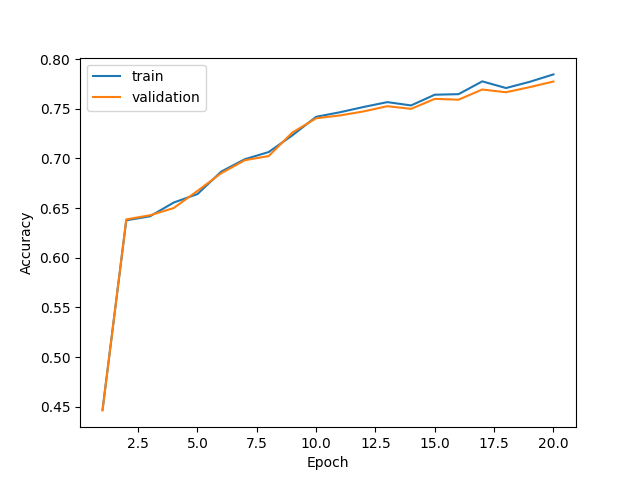
\includegraphics[width=0.8\textwidth]{"plots/mlp_validation_training.png"}
    \caption{MLP Accuracy with Learning Rate $\eta= 0.001$}
    \label{1.2.b 0.001 Plot}
\end{figure}


\begin{figure}[H]
    \centering
    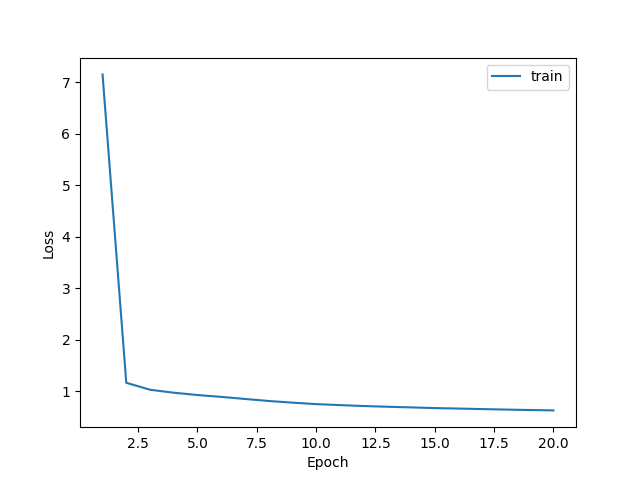
\includegraphics[width=0.8\textwidth]{"plots/mlp_loss.png"}
    \caption{MLP Loss with Learning Rate $\eta= 0.001$}
    \label{1.2.b Loss Plot}
\end{figure}

The test accuracy was 0.7505.

\section{Question 2}
Medical image classification with an autodiff toolkit.

\subsection{}

\paragraph{Answer} After running the code, the following plots were generated:

\begin{figure}[H]
    \centering
    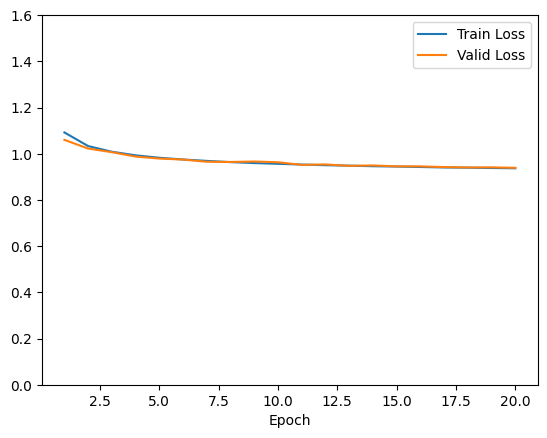
\includegraphics[width=0.8\textwidth]{"plots/logistic_regression-training-loss-batch-16-lr-0.01-epochs-20-l2-0-opt-sgd.png"}
    \caption{Training and validation loss for $\eta = 0.01$}
    \label{2.1 0.01 Loss Plot}
\end{figure}

\begin{figure}[H]
    \centering
    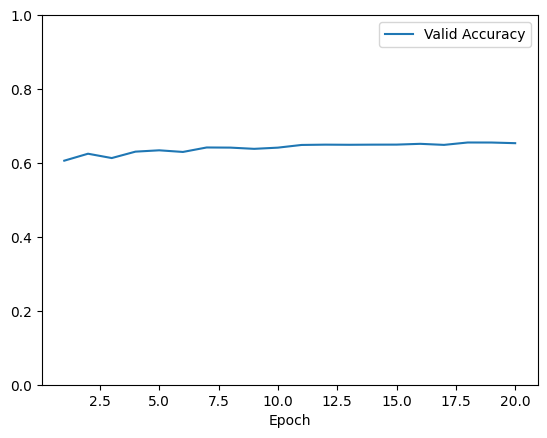
\includegraphics[width=0.8\textwidth]{"plots/logistic_regression-validation-accuracy-batch-16-lr-0.01-epochs-20-l2-0-opt-sgd.png"}
    \caption{Validation accuracy for $\eta = 0.01$}
    \label{2.1 0.01 Acc Plot}
\end{figure}

The test accuracy was 0.6200.

\subsection{}

\subsubsection{}
\paragraph{Answer} After running the code, the following plots were generated:
\begin{figure}[H]
    \centering
    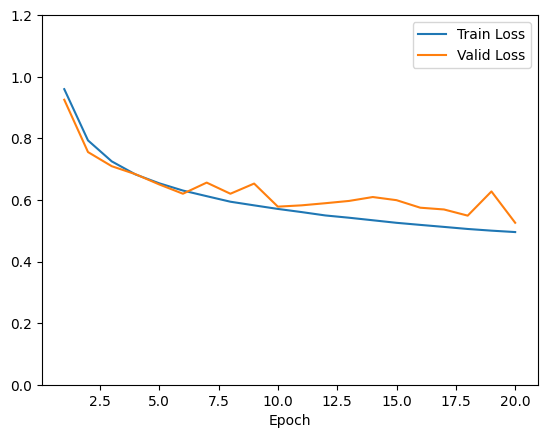
\includegraphics[width=0.8\textwidth]{"plots/mlp-training-loss-batch-16-lr-0.1-epochs-20-hidden-200-dropout-0.0-l2-0-layers-2-act-relu-opt-sgd.png"}
    \caption{Training and validation loss for batch size of 16}
    \label{2.2a batch size 16}
\end{figure}

\begin{figure}[H]
    \centering
    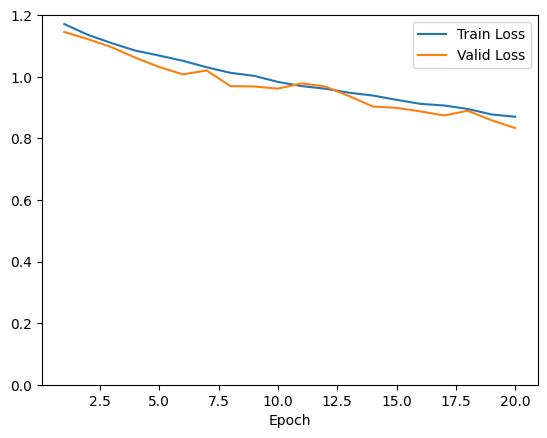
\includegraphics[width=0.8\textwidth]{"plots/mlp-training-loss-batch-1024-lr-0.1-epochs-20-hidden-200-dropout-0.0-l2-0-layers-2-act-relu-opt-sgd.png"}
    \caption{Training and validation loss for batch size of 1024}
    \label{2.2a batch size 1024}
\end{figure}

This exercise explores the trade-off between train time and performance when using different batch sizes. When training with smaller batch sizes, the model updates weights more frequently,
since each update is working with less data each time, and thus, takes more time to train when comparing to a bigger batch size. However, this frequent updating for smaller batch sizes can 
provide a regularizing effect avoiding overfitting. When compared to larger batch sizes, smaller batch sizes are more noisy, since they are more sensitive to the data they are working with. This noise can be positive, since it can help the model
to avoid converging to a local minimum and, that way, impoves the chances of finding the global minimum. On the other hand, the noise can also be negative, since it can lead to a slower convergence. On a overall note, smaller batch sizes often lead to a better 
model generalization and accuracy, despite taking more time to train. This comment can be supported by the plots above, where we can see that the model with batch size 16 has a better performance than the one with batch size 1024, despite having taken more time to train.

The best test accuracy was 0.7675 for batch size 16.

\subsubsection{}
\paragraph{Answer} After running the code, the best and worst configurations were for learning rates of 0.1 and 1, respectively:

\begin{figure}[H]
    \centering
    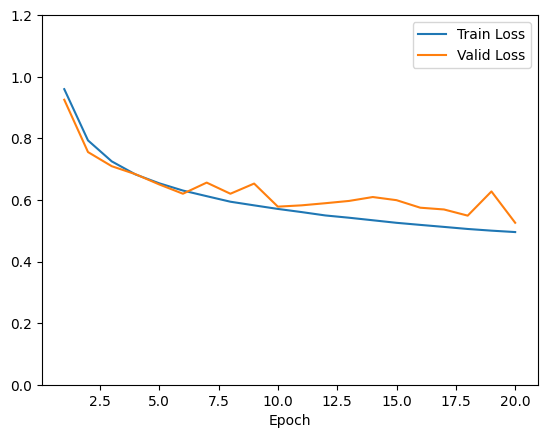
\includegraphics[width=0.8\textwidth]{"plots/mlp-training-loss-batch-16-lr-0.1-epochs-20-hidden-200-dropout-0.0-l2-0-layers-2-act-relu-opt-sgd.png"}
    \caption{Training and validation loss for learning rate of 0.1}
    \label{2.2b learning rate 0.1}
\end{figure}

\begin{figure}[H]
    \centering
    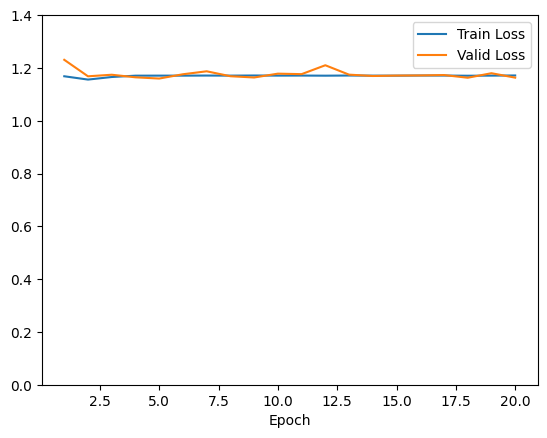
\includegraphics[width=0.8\textwidth]{"plots/mlp-training-loss-batch-16-lr-1.0-epochs-20-hidden-200-dropout-0.0-l2-0-layers-2-act-relu-opt-sgd.png"}
    \caption{Training and validation loss for learning rate of 1}
    \label{2.2b learning rate 1}
\end{figure}

This exercise explores the trade-off between a high and low learning rate. When using a high learning rate, the model converges faster, since it is taking bigger steps towards the minimum. 
However, this can lead to problems, since the model can overshoot the optimal minimum. On the other hand, when using a low learning rate, the model takes smaller steps towards 
the minimum and thus, it takes more time to converge. This can be a good thing, since it can avoid overshooting the minimum and diverging. Important to note, that for a very low learning rate,
the model can get stuck in a local minimum, not achieving the best possible accuracy. For our specific case, the model with learning rate 1 seems to have converged too quickly on a non optimal minimum,
since the model does not improve further after the first ephocs, as we can see in the Figure \ref{2.2b learning rate 1}. For the learning rates 0.01 and 0.001, since the convergence is slower, 
the model was not able to reach a good accuracy in 20 epochs. The best test accuracy was 0.7675 for learning rate 0.1, wich offered a good balance between convergence speed and accuracy, for the given number of epochs.

\subsubsection{}
\paragraph{Answer} After running the code, the best configuration was for the model with a dropout probability of 0.2 and the worst one was for the default model.

\begin{figure}[H]
    \centering
    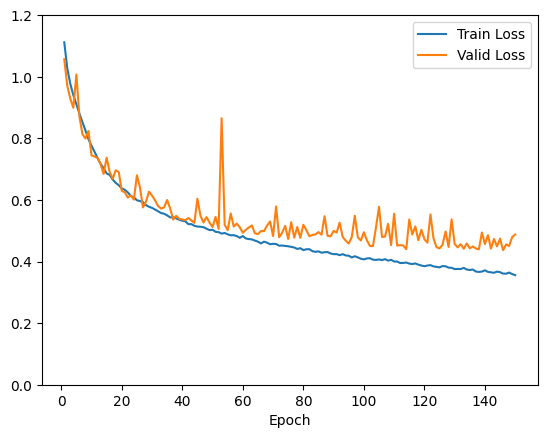
\includegraphics[width=0.8\textwidth]{"plots/mlp-training-loss-batch-256-lr-0.1-epochs-150-hidden-200-dropout-0.0-l2-0-layers-2-act-relu-opt-sgd.png"}
    \caption{Training and validation loss for default model}
    \label{2.2c default model}
\end{figure}

\begin{figure}[H]
    \centering
    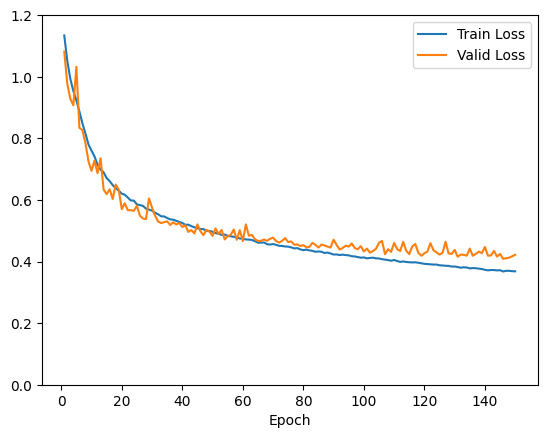
\includegraphics[width=0.8\textwidth]{"plots/mlp-training-loss-batch-256-lr-0.1-epochs-150-hidden-200-dropout-0.2-l2-0-layers-2-act-relu-opt-sgd.png"}
    \caption{Training and validation loss for model with dropout of 0.2}
    \label{2.2c dropout 0.2}
\end{figure}


For the base model proposed in this exercise, although the validation loss starts to slow down its decrease, there are no clear signs 
of overfitting. 

In this exercise, we explored two different techniques to avoid overfitting. We started by testing the model by applying L2 regularization, which adds 
a penalty term to the loss function, forcing the model to learn smaller weights, encouraging the model to find simpler solutions and, that way, reducing 
the impact of noisy or irrelevant features. 

After that we tested applying a dropout, which is a technique that randomly drops a proportion of the network's nodes during each training epoch, 
forcing the network to avoid relying too heavily on any one feature. The L2 regularization, only managed to a slight improvement in the 
validation loss's stability. On the other hand, the dropout technique, managed to significantly improve the model's performance,
as we can see in the Figure \ref{2.2c dropout 0.2}. The best test accuracy was 0.7825 for the model with dropout probability of 0.2.



\section{Question 3}

\subsection{}
\subsubsection{}
\paragraph{Answer}

To demonstrate that the specified Boolean function cannot be computed by a single perceptron, let's consider a simple case where \( D = 2 \), \( A = -1 \), and \( B = 1 \). The function \( f \) is defined as:

\[
f(x) = 
\begin{cases} 
1 & \text{if } \sum_{i=1}^{D} x_i \in [-1, 1], \\
-1 & \text{otherwise}
\end{cases}
\]

In this setup:

\begin{itemize}
    \item For \( x = (+1, +1) \), the sum \( \sum x_i = 2 \). Since 2 is not in the range [-1, 1], \( f(x) = -1 \).
    \item For \( x = (-1, -1) \), the sum \( \sum x_i = -2 \). Since -2 is also not in the range [-1, 1], \( f(x) = -1 \).
    \item For \( x = (-1, +1) \) or \( x = (+1, -1) \), the sum \( \sum x_i = 0 \). This falls within the range [-1, 1], so \( f(x) = 1 \) for these inputs.
\end{itemize}

The visual representation of the points can be seen in Figure \ref{3a Plot}. The red points represent the inputs that should be classified as \( +1 \) and the blue points represent the inputs that should be classified as \( -1 \).

The critical point here is that a single perceptron is fundamentally a linear classifier, which means it can only separate data points using a straight line in the feature space. However, in this example, there is no straight line that can separate these points accordingly in a 2D space, to satisfy the function \( f \).

This example thus serves as a counter-example proving that the given function cannot generally be computed with a single perceptron, as it requires a non-linear decision boundary which a single perceptron cannot provide. 

\begin{figure}[H]
    \centering
    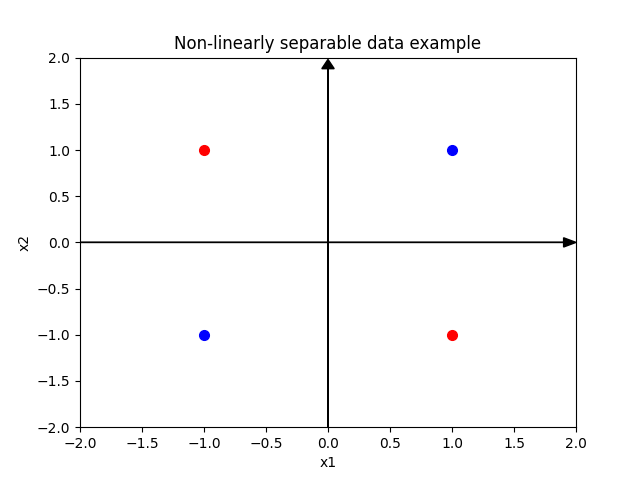
\includegraphics[width=0.8\textwidth]{"plots/3a.png"}
    \caption{Classification of points using the function \( f \)}
    \label{3a Plot}
\end{figure}
\subsubsection{}
\paragraph{Answer}

Firstly, we will start by defining the weights and biases of the network. We will use the notation
\( W^{(l)} \) and \( b^{(l)} \) to represent the weights and the biases, respectively, of the \( l \)-th layer. 
We will also use $X = \begin{bmatrix}
    x_1 & ... & x_D
\end{bmatrix}
$ to represent the input vector.

\bigskip

The idea behind the weights and biases of the first layer is that we want to verify if the sum of the input vector is within the range [A, B].
However, we have to do this individually, computing the lower bound condition for the first hidden unit, 
and the upper bound condition for the second hidden unit.

\bigskip

The innequation for the lower bound condition is:

\bigskip

$ \sum_{i=1}^{D} x_i \geq A \iff -A + \sum_{i=1}^{D} x_i \geq 0$

The innequation for the upper bound condition is:

\bigskip

$ \sum_{i=1}^{D} x_i \leq B \iff B + \sum_{i=1}^{D}- x_i \geq 0$

\bigskip

From this innequations we can derive the weights and biases of the first layer:

\bigskip

\( W^{(1)} = \begin{bmatrix}
    1  & ... & 1  \\
    -1 & ... & -1
\end{bmatrix}
\), where \(W^{(1)}\) is a matrix of size 2 x D, and D is the size of the input vector.

\(b^{(1)} = \begin{bmatrix}
    -A \\
    B
\end{bmatrix}
\), where A is the lower bound of the sum of the input vector, and B is the upper bound of the sum of the input vector. 

\bigskip

If $Z^{(1)}$ is the pre-activation of the first layer, we have that $Z^{(1)} = W^{(1)}X + b^{(1)}$ and
$Z^{(1)} = \begin{bmatrix}
    -A + \sum_{i=1}^{D} x_i\\
    B + \sum_{i=1}^{D}- x_i
\end{bmatrix}
$.

\bigskip

The first hidden unit's output will be $g(Z^{(1)}_1)$, and it will be 1 if the sum of the input vector is greater than or equal to A, 
and -1 otherwise.
The second hidden unit's output will be $g(Z^{(1)}_2)$, and it will be 1 if the sum of the input vector is less than or equal to B, 
and -1 otherwise.

This means the first hidden unit's output is 1 if the sum of the input vector respects the lower bound, 
and the second hidden unit's output is 1 if the sum of the input vector respects the upper bound.

For the second layer, we want to be able to check if both conditions were met in the hidden units. For this we have:

\bigskip

\( W^{(2)} = \begin{bmatrix}
    1 & 1
\end{bmatrix}
\).

\medskip

\(b^{(2)} = \begin{bmatrix}
    -1
\end{bmatrix}
\).

\bigskip

\(W^{(2)}\) and \(b^{(2)}\) are used to compute an AND logic function of the two hidden units. We use this since the output of
the hidden units is either -1 or 1, which can be considered boolean, and by computing the AND we can verify if they respect both the 
lower bound and upper bound and thus, belong to the range \([A, B]\). 

With this, if \(h(x)\) is the resulting function of the network, we have that \(h(x) = 1\) if the sum of the input vector is within the range \([A, B]\),
and -1 otherwise, that way \(h(x) = f(x)\), and we prove this neural network computes \(f(x)\).

\bigskip

Now we need to make sure our network is robust to infinitesimal perturbation of the inputs.
If we have an input vector $X = \begin{bmatrix}
    1
\end{bmatrix}
$, and we perturb it to make it $X' = \begin{bmatrix}
    1 + \epsilon
\end{bmatrix}
$, with $\epsilon \in \mathbb{R}$, $\epsilon > 0$ and $D = A = B = 1$, since $\epsilon$ is a really small number, 
we have that $h(X) = 1$ and $h(X') = -1$, so the current network is not robust to infinitesimal perturbation of the inputs.

\bigskip

To prevent this from happening, we need to change the interval of values we want to accept from $[A, B]$ to $[A - \epsilon, B + \epsilon]$.
Since the input vector contains only integers, we can say that
the sum of the input vector is also an integer. Hence, we need an $\epsilon$ that is smaller than 1. 

This means we have to create new inequations for the lower bound and upper bound conditions, 
and consequently we have to change the weights and biases of the first layer.

The first hidden unit needs to represent the following inequation:

\bigskip

$(\sum_{i=1}^{D} x_i) \geq A - \epsilon \iff (\sum_{i=1}^{D} x_i) - A + \epsilon \geq 0$

\bigskip

The second hidden unit needs to represent the following inequation:

\bigskip

$(\sum_{i=1}^{D} x_i) \leq B + \epsilon \iff B - (\sum_{i=1}^{D} x_i) - \epsilon \geq 0$

\bigskip

Since $\epsilon \in \mathbb{R}$ and $\epsilon > 0$, we can consider that $\epsilon = k1/k2$ (we are assuming that $\epsilon$
is a fractional number and not irrational), where $k1, k2 \in \mathbb{Z}$, 
and $k1 > 0, k2 > 0$ and $k1 < k2 (\epsilon < 1)$. This way we can rewrite the inequations as:

\bigskip

$(\sum_{i=1}^{D} x_i) - A + k1/k2 \geq 0 \iff k2(\sum_{i=1}^{D} x_i) - k2A + k1 \geq 0$

\bigskip

$B - (\sum_{i=1}^{D} x_i) - k1/k2 \geq 0 \iff k2B - k2(\sum_{i=1}^{D} x_i) - k1 \geq 0$

\bigskip

This way, we can rewrite the weights and biases of the first layer as:

\bigskip

\( W^{(1)} = \begin{bmatrix}
    k2  & ... & k2  \\
    -k2 & ... & -k2
\end{bmatrix}
\)

\medskip

\(b^{(1)} = \begin{bmatrix}
    -k2A + k1 \\
    k2B - k1
\end{bmatrix}
\)

\bigskip

If $Z^{(1)}$ is the pre-activation of the first layer, we have that $Z^{(1)} = W^{(1)}X + b^{(1)}$ and
$Z^{(1)} = \begin{bmatrix}
    k2(\sum_{i=1}^{D} x_i) - k2A + k1\\
    k2B - k2(\sum_{i=1}^{D} x_i) - k1
\end{bmatrix}
$.

\bigskip

With this, we have that the first hidden unit's output will be $g(Z^{(1)}_1)$, and it will be 1 if the sum of the 
input vector is greater than or equal to A - $\epsilon$, and -1 otherwise. The second hidden unit's output will be $g(Z^{(1)}_2)$,
and it will be 1 if the sum of the input vector is less than or equal to B + $\epsilon$, and -1 otherwise.

A possible set of values for $k1$ and $k2$ is $k1 = 1$ and $k2 = 10$. With this, $\epsilon = 0.1$, and we accept values in
the range $[A - \epsilon, B + \epsilon] = [A - 0.1, B + 0.1]$.

With this, the first hidden unit's output is 1 if the sum of the input vector respects the lower bound ($A - 0.1$),
and the second hidden unit's output is 1 if the sum of the input vector respects the upper bound ($B + 0.1$).

The second layer remains the same, since we want to compute the AND logic function of the two hidden units, and since the output of
the hidden units is either -1 or 1, which can be considered boolean, we can compute the AND logic function of the two hidden units.

\bigskip

With this, we have that \(h(x) = f(x)\), and the network is robust to infinitesimal perturbation of the inputs, since it now accepts inputs
that are within the range \([A - \epsilon, B + \epsilon]\).

\subsubsection{}

\paragraph{Answer}

The rectified linear unit (ReLU) activation function is defined as:

\[ 
    ReLU(x) = 
    \begin{cases}
        x & x \geq 0, \\
        0 & \text{otherwise}
    \end{cases}
\]

First, we will start by defining the weights and biases of the network. We will use the same notation as the previous 
exercise for the weights and biases.

\bigskip

The idea behind the weights and biases of the first layer is somewhat the opposite of the first exercise, since this time we want our innequations
to use $\leq 0$ instead of $\geq 0$. We want the hidden units to output 0 if the sum of the input vector respects one of the bounds, 
and a positive value otherwise (first branch of the ReLU).

But like in the previous exercise, we must do this individually, computing the lower bound condition for the first hidden unit, 
and the upper bound condition for the second hidden unit, same as the previous exercise.

\bigskip

For this we have to use the weights and biases to represent the inequations that represent the bound but with less or equal to 0, in order for
the ReLU output to be 0:

\bigskip

$ \sum_{i=1}^{D} x_i \geq A \iff -A + \sum_{i=1}^{D} x_i \geq 0 \iff -(\sum_{i=1}^{D} x_i) + A \leq 0$.

\medskip

$ \sum_{i=1}^{D} x_i \leq B \iff -B + \sum_{i=1}^{D} x_i \leq 0$.

\bigskip

To represent these inequations with weights and biases, we have:

\bigskip

\( W^{(1)} = \begin{bmatrix}
    -1 & ...  & -1\\
    1 & ... & 1
\end{bmatrix}
\), where \(W^{(1)}\) is a matrix of size 2 x D, and D is the size of the input vector.

\bigskip

\(b^{(1)} = \begin{bmatrix}
    A\\
    -B
\end{bmatrix}
\), where A is the lower bound of the sum of the input vector, and B is the upper bound of the sum of the input vector.

\bigskip

Let's consider $Z^{(1)}$ as the pre-activated output of the first layer. This means $Z^{(1)} = W^{(1)}X + b^{(1)}$, and
$Z^{(1)} = \begin{bmatrix}
    A -\sum_{i=1}^{D} x_i\\
    -B + \sum_{i=1}^{D} x_i
\end{bmatrix}
$.

\bigskip

The first hidden unit's pre-activated output will be $g(Z_1^{(1)})$, and the hidden unit's activated output 
will be 0 if the sum of the input vector is greater than or equal to A, and a positive value ($Z_1^{(1)}$) otherwise.

The second hidden unit's output will be $g(Z_2^{(1)})$, and it will be 0 if the sum of the input vector is less than or equal to B, 
and a positive value ($Z_2^{(1)}$) otherwise.

This means the first hidden unit's output is 0 if the sum of the input vector respects the lower bound, 
and the second hidden unit's output is 0 if the sum of the input vector respects the upper bound.

\bigskip

For the second layer, we want only to accept values that respect both bounds, so we use our weights and biases to verify if any of the values
of the hidden layer are positive, and if they are, we want to output -1, because it means one of the bounds was not respected.

\bigskip

For this we have:

\bigskip

\( W^{(2)} = \begin{bmatrix}
    -1 & -1
\end{bmatrix}
\).

\bigskip

\(b^{(2)} = \begin{bmatrix}
    -1
\end{bmatrix}
\).

\bigskip

The idea behind \(W^{(2)}\) and \(b^{(2)}\) is to compute a function similar to the logic AND, but since this time our inputs are not in 
\{-1, 1\}, we cannot use the weights used in the previous exercise.
Since each hidden unit outputs 0 if the sum of the input vector respects one of the bounds, and a positive value otherwise, we can set the 
weights of the second layer as -1's, and the bias as 0, so that the pre-activated output of the network is 0 if the sum of the input vector 
respects both bounds, and a negative value otherwise.

\bigskip

Since the pre-activated output this time is not in \{-1, 1\}, we need to apply an activation function to the pre-activated output of the network. 
For this we can use the sign function, which will output 1 if the pre-activated output is positive or zero, and -1 otherwise.

Since when an input vector respects both bounds, the pre-activated output of the network is 0, the sign function will output 1. If the input doesn't
respect both bounds, the pre-activated output of the network will be negative, and the sign function will output -1.

With this, if h(x) is the resulting function of the network, we have that h(x) = 1 if the sum of the input vector is within the range [A, B], 
and -1 otherwise, and, thus, h(x) = f(x), and we prove this neural network computes f(x).

\bigskip

To ensure that our network is robust to infinitesimal perturbation of the inputs, we need to do something similar to what we did in the previous exercise.

We need to ensure that the weights and biases of the first layer are such that the hidden units output 0 if the sum of the input vector is 
within the range [A - $\epsilon$, B + $\epsilon$], and a positive value otherwise.

This means we have to create new inequations for the lower bound and upper bound conditions, 
and thus we have to change the weights and biases of the first layer.

\bigskip

The first hidden unit needs to represent the following inequation:

\bigskip

$ \sum_{i=1}^{D} x_i \geq A - \epsilon \iff -A + \epsilon + \sum_{i=1}^{D} x_i \geq 0 
\iff -(\sum_{i=1}^{D} x_i) + A - \epsilon \leq 0$

\bigskip

The second hidden unit needs to represent the following inequation:

\bigskip

$ \sum_{i=1}^{D} x_i \leq B + \epsilon \iff -B - \epsilon + \sum_{i=1}^{D} x_i \leq 0$

\bigskip

Since $\epsilon \in \mathbb{R}$ and $\epsilon > 0$, we can consider that $\epsilon = k1/k2$ (we are assuming that $\epsilon$
is a fractional number and not irrational), where $k1, k2 \in \mathbb{Z}$, and $k1 > 0, k2 > 0$ and $k1 < k2 (\epsilon < 1)$.

\bigskip

This way we can rewrite the inequations as:

\bigskip

$ -(\sum_{i=1}^{D} x_i) + A - k1/k2 \leq 0 \iff -k2(\sum_{i=1}^{D} x_i) + k2A - k1 \leq 0$

\bigskip

$ -B - k1/k2 + \sum_{i=1}^{D} x_i \leq 0 \iff -k2B + k2(\sum_{i=1}^{D} x_i) + k1 \leq 0$

\bigskip

This way, we can rewrite the weights and biases of the first layer as:

\bigskip

\( W^{(1)} = \begin{bmatrix}
    -k2 & ...  & -k2\\
    k2 & ... & k2
\end{bmatrix}
\)

\bigskip

\(b^{(1)} = \begin{bmatrix}
    k2A - k1 \\
    -k2B + k1
\end{bmatrix}
\)

\bigskip

If $Z^{(1)}$ is the pre-activation of the first layer, we have that $Z^{(1)} = W^{(1)}X + b^{(1)}$ and
$Z^{(1)} = \begin{bmatrix}
    -k2(\sum_{i=1}^{D} x_i) + k2A - k1\\
    -k2B + k2(\sum_{i=1}^{D} x_i) + k1
\end{bmatrix}
$.

\bigskip

With this, we have that the first hidden unit's output will be $g(Z^{(1)}_1)$, and it will be 0 if the sum of the 
input vector is greater than or equal to A - $\epsilon$, and a positive value ($Z^{(1)}_1$) otherwise. 
The second hidden unit's output will be $g(Z^{(1)}_2)$, and it will be 0 if the sum of the input vector is less than or equal 
to B + $\epsilon$, and a positive value ($Z^{(1)}_2$) otherwise.

A possible set of values for $k1$ and $k2$ is $k1 = 1$ and $k2 = 10$. With this, $\epsilon = 0.1$, and we accept values in
the range $[A - \epsilon, B + \epsilon] = [A - 0.1, B + 0.1]$.

This means the first hidden unit's output is 0 if the sum of the input vector respects the lower bound ($A - 0.1$),
and the second hidden unit's output is 0 if the sum of the input vector respects the upper bound ($B + 0.1$).

\bigskip

The second layer remains the same, since we want to compute the AND logic function of the two hidden units, and since the output of
the hidden units is either -1 or 1, which can be considered boolean, we can compute the AND logic function of the two hidden units.

With this, we have that \(h(x) = f(x)\), and the network is robust to infinitesimal perturbation of the inputs, since it now accepts inputs
that are within the range \([A - \epsilon, B + \epsilon]\).

\section{Credits}

Frederico did everything.
Sebastião did nothing, didn't even know how to make an empty line in latex.
Fim da 15, inicio da 16.

\end{document}
